\chapter{VAE Results}
\label{chap:8_vae_evaluation_studies}
In this section, we will briefly evaluate the the performance of our VAE model in regards to its reconstruction ability. We aim to explore the effects of the different modifications to the loss function, as presented in \cref{subsec:5_vae_reconstruction}. To do this, we will begin with a plain reconstruction error, before adding a depth weighting, and finally edge loss.
Moreover, we explore these implementations to both MSE and BCE loss.

An overview of the best models with their modified losses, best epoch and their time-to-train is shown below:
\begin{table}[hbt]
    \centering
    \begin{tabular}{||c|c|c|c||}
    \hline
        ID & Model & Epoch & Time \\
    \hline\hline
        1 & Vanilla MSE & 40 & 19h 4m \\\hline
        2 & Vanilla BCE & 50 & 1d 14h 36m \\\hline
        3 & Depth Weighted MSE & 60 & 3d 4h 52m \\\hline
        4 & Depth Weighted BCE & 60 &  1d 13h 54m \\\hline
        5 & Depth Weighted MSE with Edge Loss & 100 & 1d 22h 49m \\\hline
        6 & Depth Weighted BCE with Edge Loss & 100 & 3d 3h 37m \\
    \hline
    \end{tabular}
    \caption{List of VAE models.}
    \label{tab:8_all_vae_models}
\end{table}


\section{Training}
\label{sec:8_training}
We train our networks on 202,558 depth images for 100 epochs, where we present their training and test plots. We also train these two at a time, which slightly reduces their training times. 
Overall, not much can be seen from the training plots, apart from ensuring that training is stable and the models do not over-fit. Normally, the approach would be to compare the losses of each side by side, but since the scale of the losses are dissimilar, we provide this as an indication of how the changes to the reconstruction affect the loss values and training plots. 


\subsection{Vanilla Loss Function}
\label{sec:8_vanilla}
Beginning first with the vanilla reconstruction loss, the overall loss function for a batch $B$ of $m$ of samples is: 
\begin{equation}
    \widetilde{\loss}_B\,(\boldsymbol{\theta}, \boldsymbol{\phi}; \d^{(i)}, {\d^f}^{(i)} ) =
    \frac{1}{m} \sum_{i=1}^m
    \Bigg(
    \log \pbt ({\d^f}^{(i)} |\, \bz^{(i,l)}) 
    -
    \DKL{\qbp(\bz |\, \d^{(i)})}{\log \pbt(\bz)}
    \Bigg)
    \label{eq:8_vanilla_loss_estimator_batch}
\end{equation}
Then, the reconstruction loss $\loss^{(i)}_{\text{REC}} = \log \pbt (\boldsymbol{\hat{d}^f}^{(i)} |\, \bz^{(i,l)})$ can be replaced with the vanilla MSE and BCE, which is implemented in practice as:
\begin{equation}
    \loss^{(i)}_{\text{MSE}} = \norm{\, \boldsymbol{\hat{d}^f}^{(i)} - \boldsymbol{d^f}^{(i)}}
    \label{eq:8_mse_vanilla_loss}
\end{equation}
\begin{equation}
    \loss^{(i)}_{\text{BCE}} =\boldsymbol{d^f}^{(i)} \log \sigmoid{\boldsymbol{\hat{d}^f}^{(i)}} +  (1 - \boldsymbol{d^f}^{(i)}) \log \sigmoid{1 - \boldsymbol{\hat{d}^f}^{(i)}}
    \label{eq:8_bce_vanilla_loss}
\end{equation}
where $\sigma$ is used to denote the \textit{sigmoid} activation function. With this, we present the training curves in \cref{fig:8_vanilla_vae}.
\begin{figure}[htb]
    \centering
    \begin{subfigure}[b]{\textwidth}
        \centering
        \captionsetup{justification=centering}
        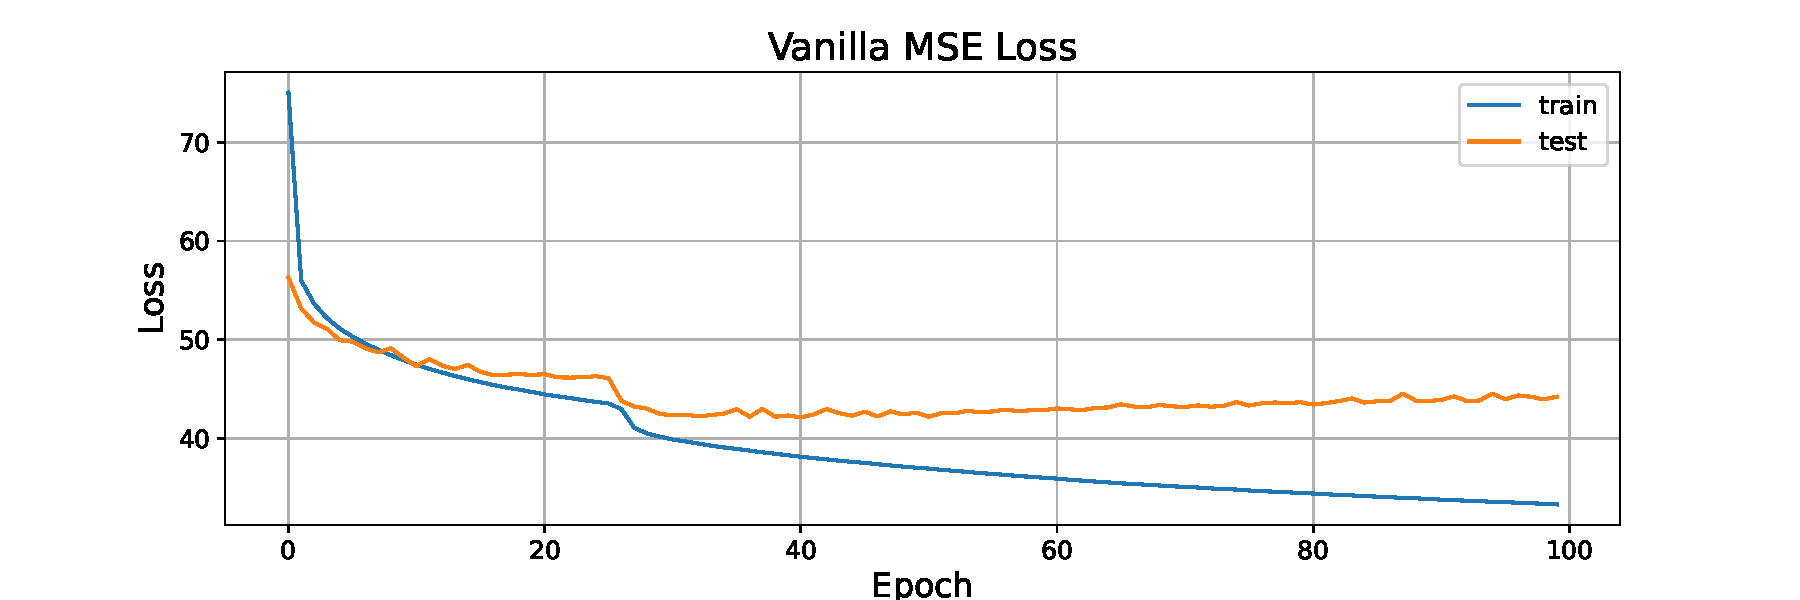
\includegraphics[width=0.99\textwidth]{figures/8_/1_final_MSE_plain.pdf}
        \label{fig:1_final_MSE_plain}
    \end{subfigure} \\
    \begin{subfigure}[b]{\textwidth}
        \centering
        \captionsetup{justification=centering}
        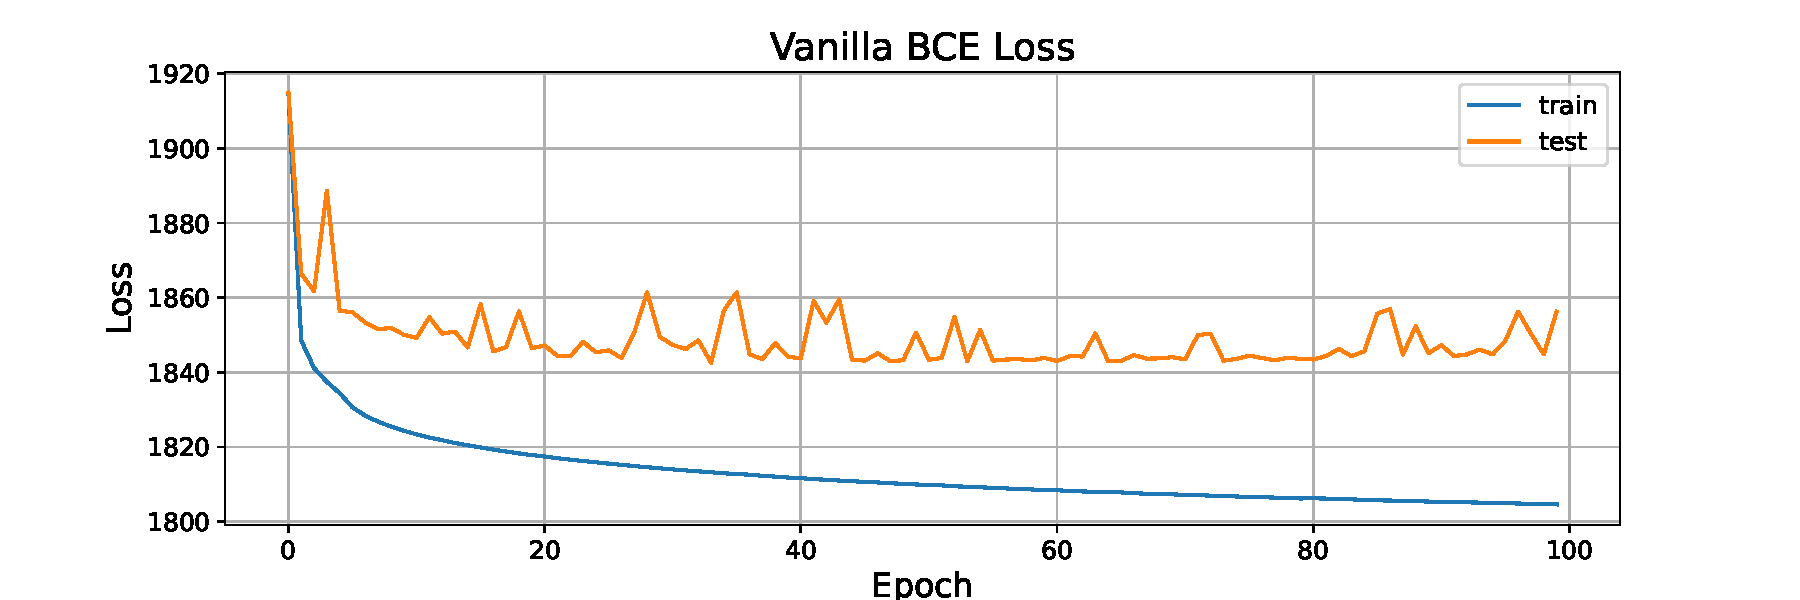
\includegraphics[width=0.99\textwidth]{figures/8_/4_final_BCE_plain.pdf}
        \label{fig:4_final_BCE_plain}
    \end{subfigure} 
    \caption{Training and test loss for the vanilla MSE and BCE models.}
    \label{fig:8_vanilla_vae}
\end{figure}
From the figures, we observe a slight over-fitting for both models, where the MSE begins to over-fit beyond 40 epochs, and the BCE around 50. 

\subsection{Depth Weighted Loss}
\label{sec:8_depth}
With the vanilla models trained, we now implement the depth weighting according to the input depth image $\boldsymbol{d^f}^{(i)}$:
\begin{equation}
    \loss^{(i)}_{\text{MSE}} =  K_\text{depth}(\boldsymbol{d^f}^{(i)}) \cdot \norm{\, \boldsymbol{\hat{d}^f}^{(i)} - \boldsymbol{d^f}^{(i)}}
    \label{eq:8_mse_depth_weighted_loss}
\end{equation}
\begin{equation}
    \loss^{(i)}_{\text{BCE}} = K_\text{depth}(\boldsymbol{d^f}^{(i)}) \cdot \Bigg( \boldsymbol{d^f}^{(i)} \log \sigmoid{\boldsymbol{\hat{d}^f}^{(i)}} +  (1 - \boldsymbol{d^f}^{(i)}) \log \sigmoid{1 - \boldsymbol{\hat{d}^f}^{(i)}} \Bigg)
    \label{eq:8_bce_depth_weighted_loss}
\end{equation}
where the depth gain $K_\text{depth}$ is given by \cref{eq:5_depth_gain}. Using this loss, we train our models to obtain the plots in \cref{fig:8_depth_vae}.
\begin{figure}[htb]
    \centering
    \begin{subfigure}[b]{\textwidth}
        \centering
        \captionsetup{justification=centering}
        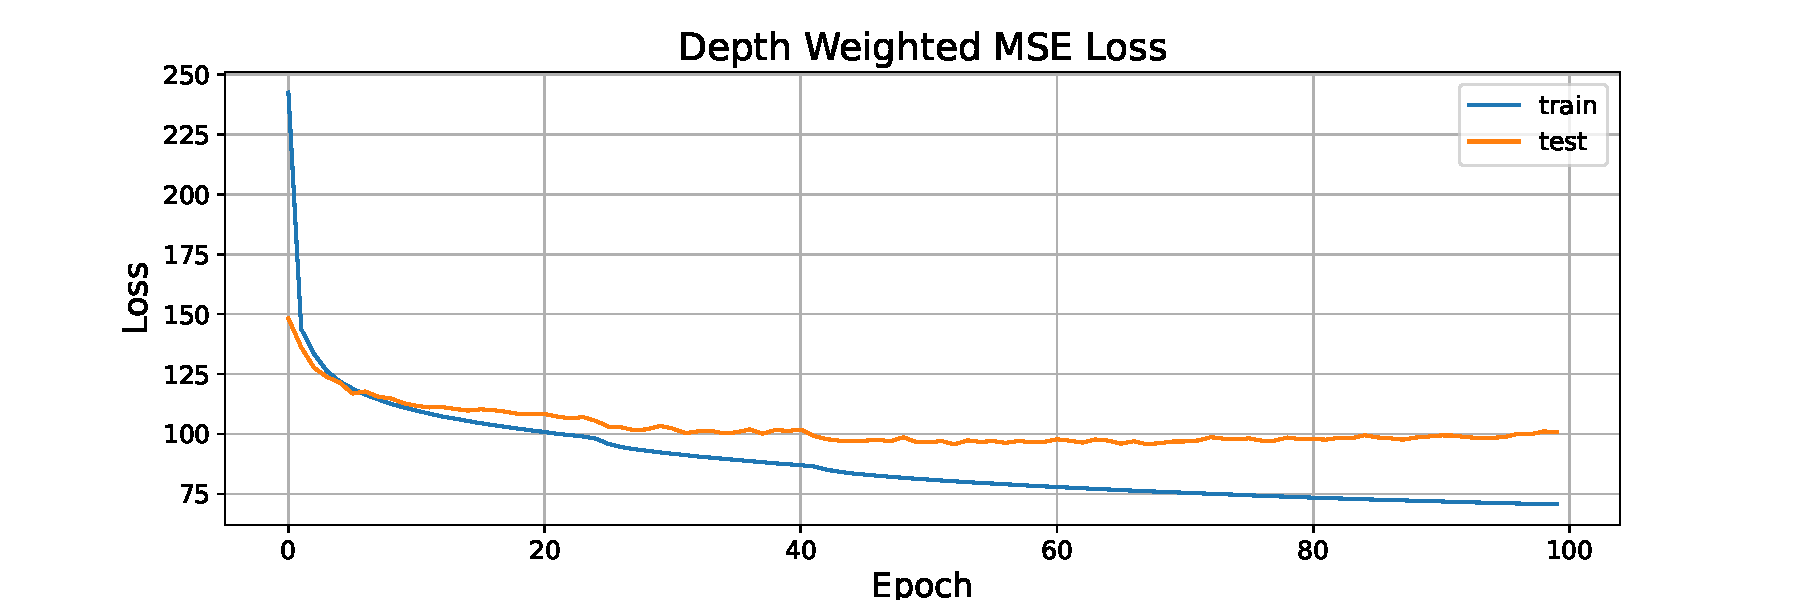
\includegraphics[width=0.99\textwidth]{figures/8_/2_final_MSE_depth_weighted10.pdf}
        \label{fig:2_final_MSE_depth_weighted10}
    \end{subfigure} \\
    \begin{subfigure}[b]{\textwidth}
        \centering
        \captionsetup{justification=centering}
        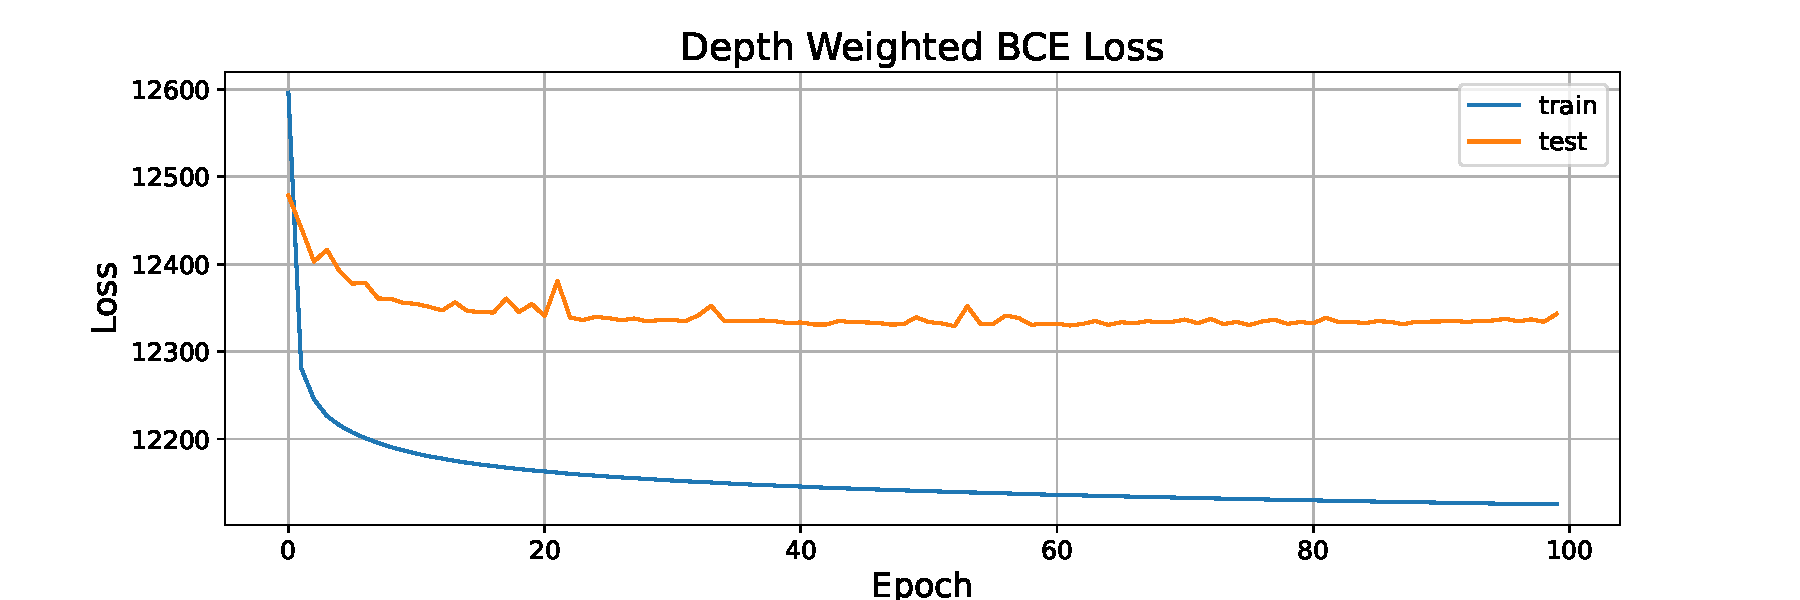
\includegraphics[width=0.99\textwidth]{figures/8_/5_final_BCE_depth_weighted10.pdf}
        \label{fig:5_final_BCE_depth_weighted10}
    \end{subfigure} 
    \caption{Training and test loss for the depth weighted MSE and BCE models.}
    \label{fig:8_depth_vae}
\end{figure}
Following a very close pattern with the vanilla training plots, we observe essentially a doubling in the total loss for the MSE, while the BCE loss increases by a factor of 10. Otherwise, both models also show a slight tendency of over-fitting, at around 60 epochs. 

\subsection{Depth Weighted Loss With Edge Loss}
\label{sec:8_edge_depth}
Finally, to implement the depth weighted losses with edge loss, we add the mean absolute error (MAE) between the edges of the depth filtered image and reconstruction:
\begin{equation}
    \loss^{(i)}_{\text{MSE}} = K_\text{depth} \cdot \boldsymbol{d^f}^{(i)} \cdot \Bigg (\norm{\, \boldsymbol{\hat{d}^f}^{(i)} - \boldsymbol{d^f}^{(i)}}_2 
    + \loss^{(i)}_{\text{edge}}
    \Bigg)
    \label{eq:8_mse_edge_depth_weighted_loss}
\end{equation}
\begin{equation}
    \loss^{(i)}_{\text{BCE}} =  K_\text{depth} \cdot \boldsymbol{d^f}^{(i)} \cdot \Bigg( \bigg(\boldsymbol{d^f}^{(i)} \log \sigmoid{\boldsymbol{\hat{d}^f}^{(i)}} +  (1 - \boldsymbol{d^f}^{(i)}) \log \sigmoid{1 - \boldsymbol{\hat{d}^f}^{(i)}} \bigg) 
    + \loss^{(i)}_{\text{edge}}
    \Bigg)
    \label{eq:8_bce_edge_depth_weighted_loss}
\end{equation}
where the edge loss is given by:
\begin{equation}
    \loss^{(i)}_{\text{edge}} = K_\text{edge} \cdot E\Big(\boldsymbol{d^f}^{(i)}\Big) \cdot \norm{\, \boldsymbol{\hat{d}^f}^{(i)} - \boldsymbol{d^f}^{(i)}}_1
\end{equation}
\begin{figure}[htb]
    \centering
    \begin{subfigure}[b]{\textwidth}
        \centering
        \captionsetup{justification=centering}
        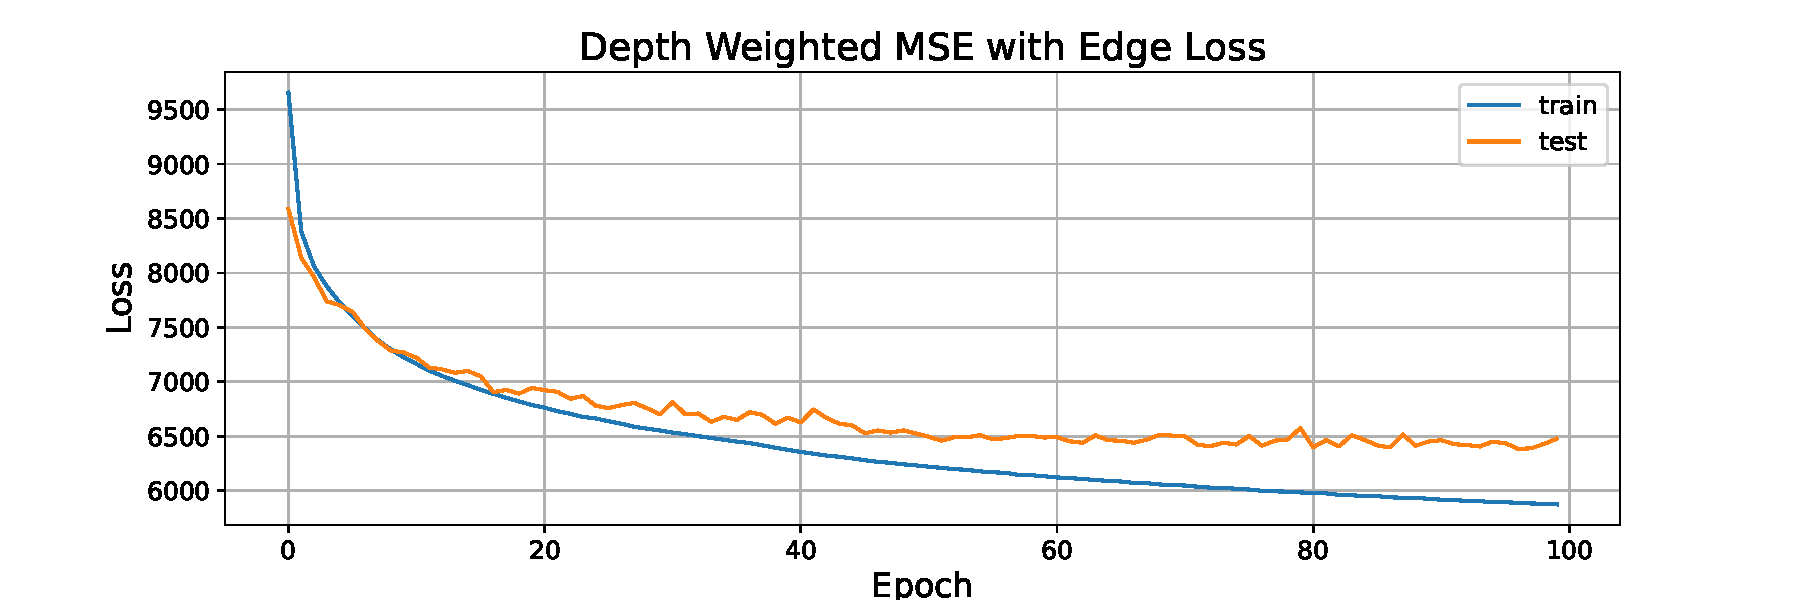
\includegraphics[width=0.99\textwidth]{figures/8_/3_final_MSE_depth_weighted10_with_depth_weighted_canny_edge_mae100_loss.pdf}
        \label{fig:3_final_MSE_depth_weighted10_with_depth_weighted_canny_edge_mae100_loss}
    \end{subfigure} \\
    \begin{subfigure}[b]{\textwidth}
        \centering
        \captionsetup{justification=centering}
        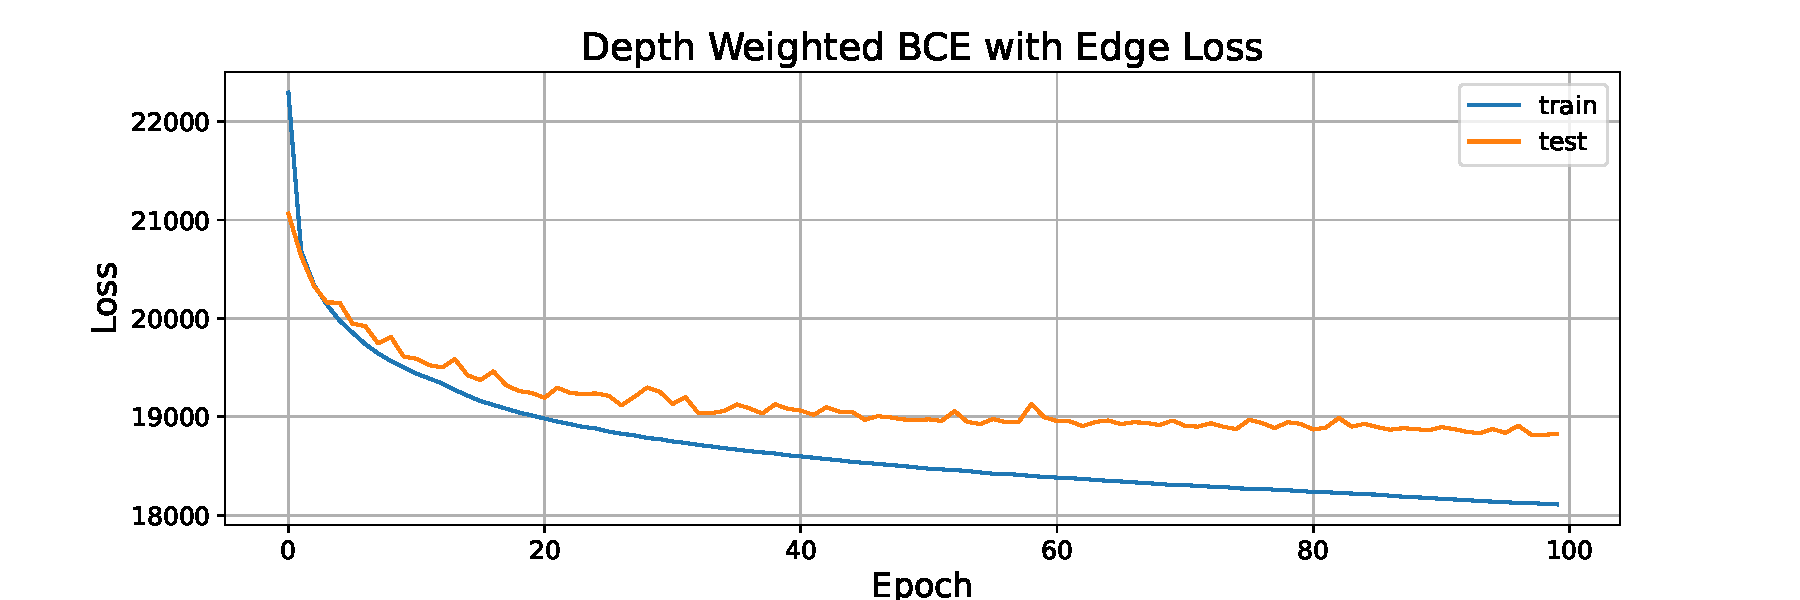
\includegraphics[width=0.99\textwidth]{figures/8_/6_final_BCE_depth_weighted10_with_depth_weighted_canny_edge_mae100_loss.pdf}
        \label{fig:6_final_BCE_depth_weighted10_with_depth_weighted_canny_edge_mae100_loss}
    \end{subfigure} 
    \caption{Training and test loss for the depth weighted MSE and BCE models when adding an edge loss term.}
    \label{fig:8_edge_depth_weighted_vae}
\end{figure}
where $E\Big(\boldsymbol{d^f}^{(i)}\Big)$ is a function that finds the edge pixels of the filtered depth image through a canny edge detector \cite{canny_edge_detection}, applies a Gaussian filter over it, and masks all values over 0 as edges. We also choose the edge gain to be $K_\text{edge} = 100$. Training our models for a final time yields the plots in \cref{fig:8_edge_depth_weighted_vae}.
Unlike the previous training plots, the MSE and BCE test loss does not increase even to 100 epochs, indicating that our model is not over-fitting our input data. Otherwise, we see that the addition of the MAE term adds a loss value of about 6000 to both MSE and BCE plots. 

\section{Testing}
\label{sec:8_testing}
So, from the training plots, it is hard to deduce the reconstruction ability of the VAE. This is because we judge this metric quite qualitatively, such that one must instead simply inspect the images either throughout or at the end of the training process. With this, we can examine the reconstruction ability of all models in \cref{fig:8_all_vae}.
\begin{figure}[htb]
    \centering
    \begin{subfigure}[b]{0.3\textwidth}
        \centering
        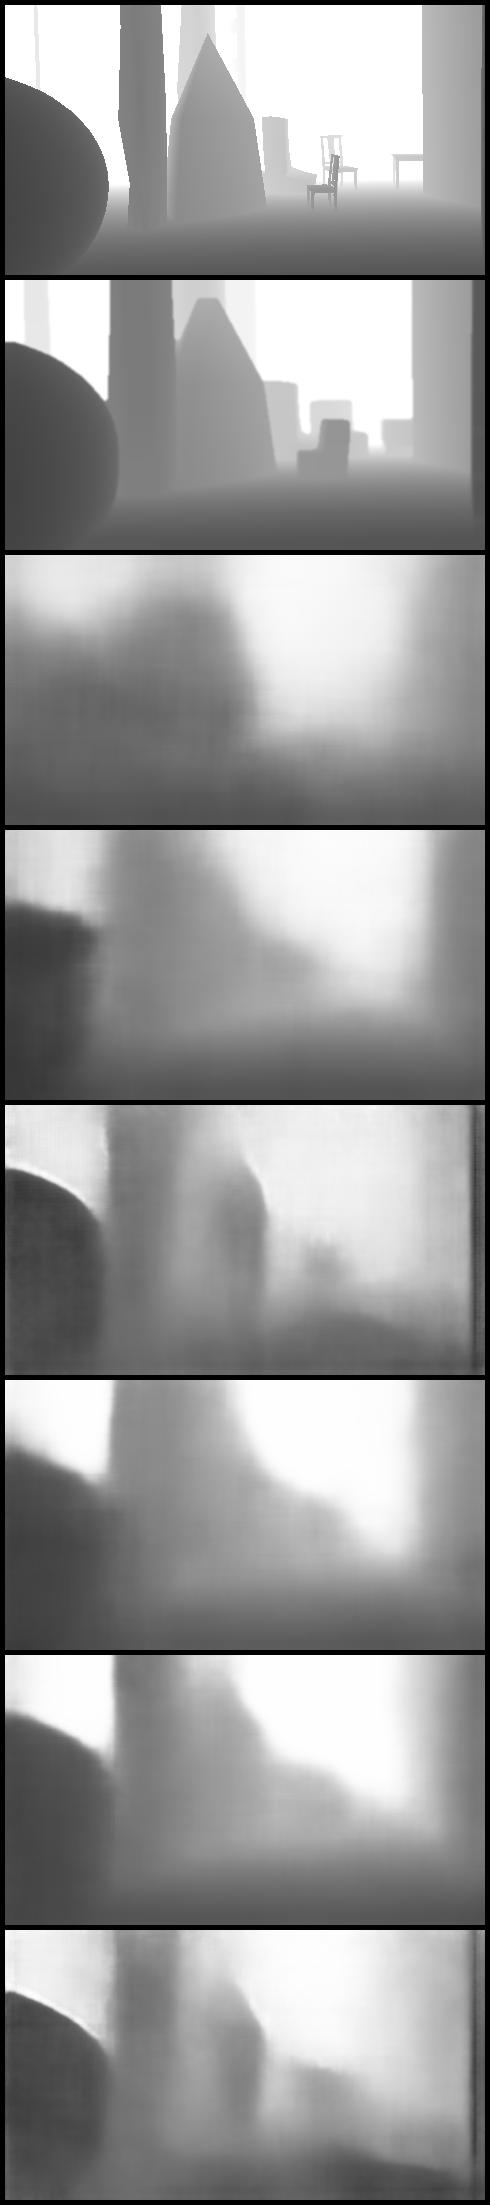
\includegraphics[height=\textheight]{figures/8_/the_same_4.jpg}
        \caption{Caption}
        \label{fig:the_same_4}
    \end{subfigure} 
    \hfill
    \begin{subfigure}[b]{0.3\textwidth}
        \centering
        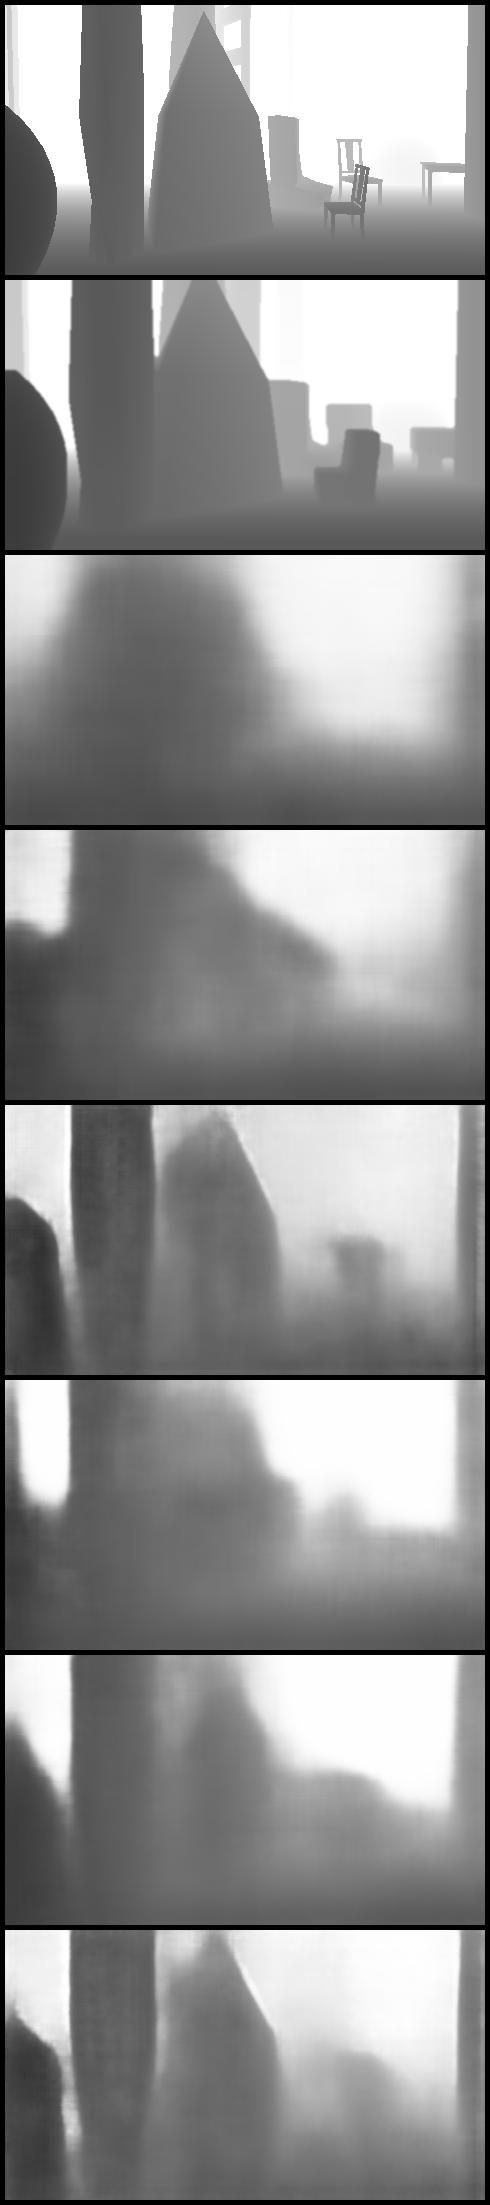
\includegraphics[height=\textheight]{figures/8_/the_same_8.jpg}
        \caption{Caption}
        \label{fig:the_same_14}
    \end{subfigure} 
    \hfill
    \begin{subfigure}[b]{0.3\textwidth}
        \centering
        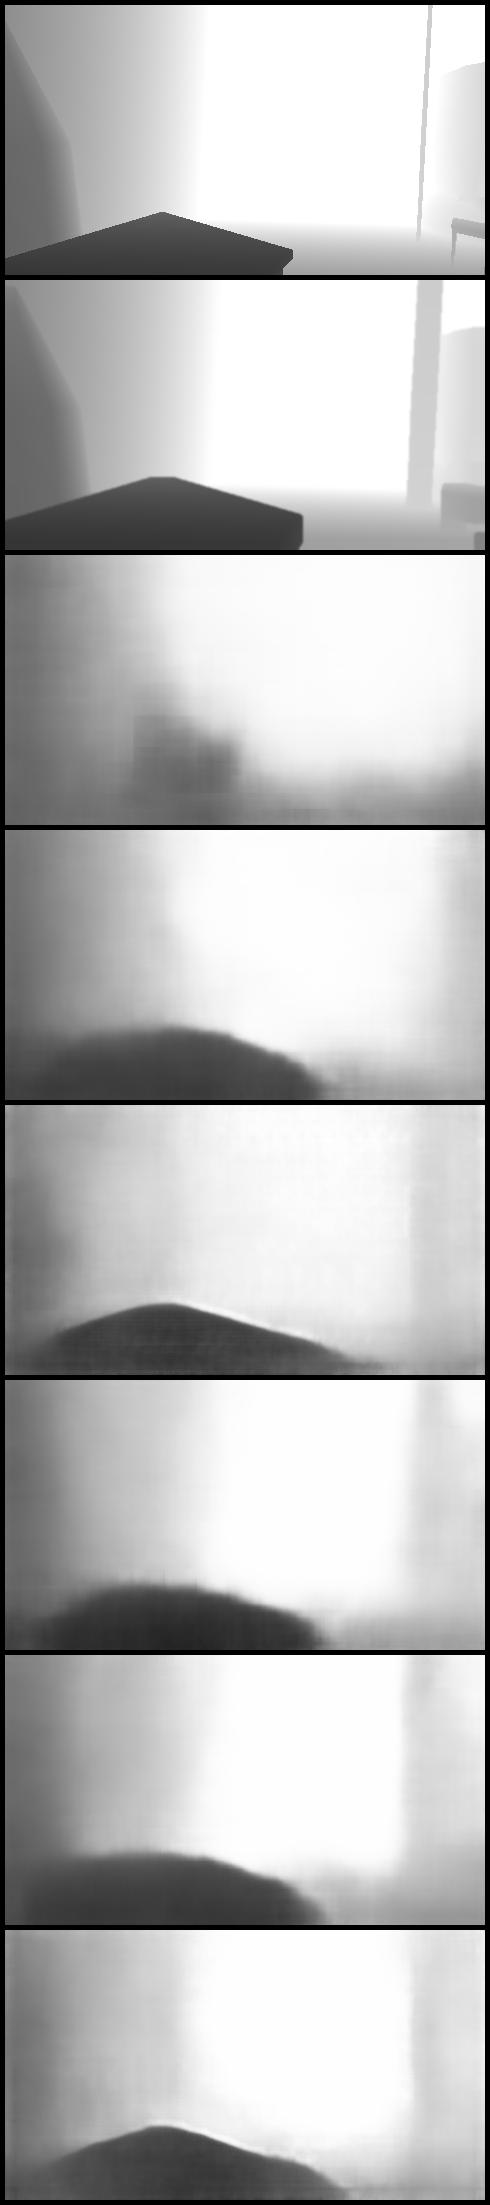
\includegraphics[height=\textheight]{figures/8_/the_same_289.jpg}
        \caption{Caption}
        \label{fig:the_same_289}
    \end{subfigure} 
    \caption{Viewing the some sample reconstructions of our trained models. The downwards order of images are: 1) Input 2) Target 3) Vanilla MSE 4) Vanilla BCE 5) Depth weighted BCE 6) Depth weighted MSE 7) Depth weighted MSE with edge loss 8) Depth weighted BCE with edge loss. Note the flipped order for 5) and 6).}
    \label{fig:8_all_vae}
\end{figure}

From the figure, we can note very clear differences in the different loss functions, and also a difference from using MSE compared to BCE as loss functions. We see first that the reconstructions for the vanilla loss functions are much more blur than the depth weight ones, even when we do not add the edge weight. This can be explained by the fact that we consider the `blurness' as an inability to reconstruct objects -- in this case obstacles -- in images. However, all objects in the scene have a depth that is much closer than the background, such that if we weight the the loss according to the closeness of pixels, the VAE be motivated to reconstruct obstacles with a higher fidelity. 

Moving onwards, we see that by adding edge losses to the depth images, we confirm our expectations that we obtain clearer edges along close obstacles to some degree. This is most prevalent for the MSE reconstructions 6) and 7), where we see that the middle pillar depth is more accurately captured than the non-edge-loss one. 

Another big difference is that of the BCE and MSE plots, where we see that the BCE loss performs much better overall in terms of clarity. However, the we can also note BCE plots also assume obstacles are closer than what they actually are, in we look at plots 5) and 8) and observe the colour of the middle grey pillar. Nonetheless, for the purpose of collision avoidance, we chose the last model, the depth weighted BCE with edge loss to serve as our inference network for our model.

















\begin{figure}
    \centering
    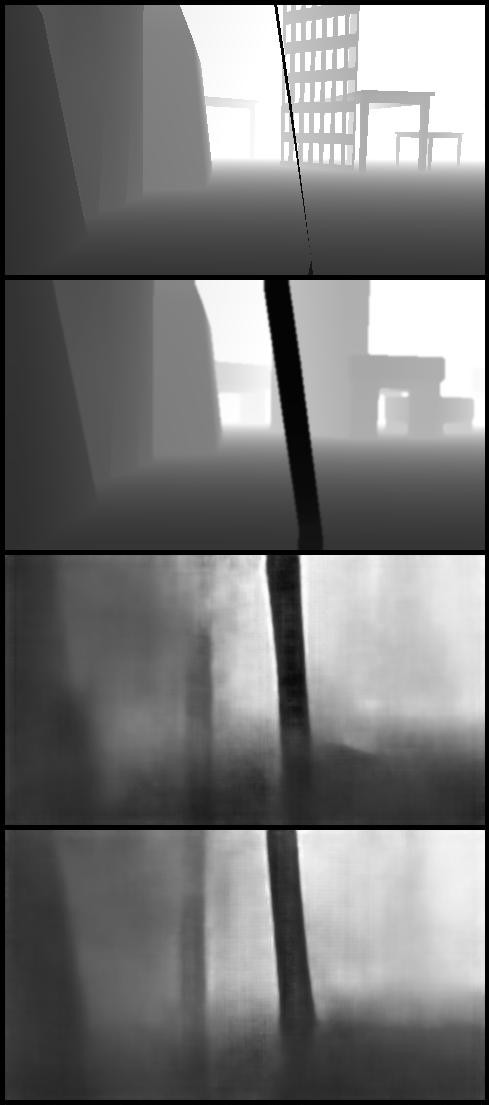
\includegraphics[width=0.5\textwidth]{figures/8_/thin.jpg}
    \caption{Reconstruction of a thin wire observed in our training dataset. We choose the two MSE and BCE models with edge loss, corresponding to the third and fourth reconstruction respectively. }
    \label{fig:thin}
\end{figure}